\documentclass[11pt]{article}
\usepackage[utf8]{inputenc}
\usepackage[T1]{fontenc}
\usepackage{hyperref}
\usepackage{url}
\usepackage{booktabs}
\usepackage{graphicx}
\usepackage{amsmath}
\usepackage{amssymb}
\usepackage{algorithm}
\usepackage{algorithmic}
\usepackage{geometry}
\geometry{margin=1in}

\title{Harness-Agnostic Skill Routing: A Two-Tier Architecture for Cross-Harness Agent Tool Selection}

\author{
  Lavya Tandel\\
  Independent Researcher\\
  \texttt{lavyatandel@gmail.com}\\
  \url{https://github.com/LavyaTandel/agent-stack-research}
}

\date{\today}

\begin{document}

\maketitle

\begin{abstract}
Large language model (LLM) agents rely on skills---structured tool descriptions loaded at runtime---to extend their capabilities. Loading all skills consumes prohibitive tokens, while loading too few risks missing critical tools. We present a two-tier skill routing architecture combining fast keyword matching with TF-IDF cosine similarity, selecting relevant skills in <1ms on CPU with 97.2\% token savings compared to full-body loading. Our system is harness-agnostic: a single registry works across OpenCode, Claude Code, and Codex. Evaluated on a 50-task benchmark spanning five domains, our approach achieves 60\% Hit@1 and 74\% Hit@5 with zero GPU and zero training. We release our registry format, router implementation, and benchmark as open source.
\end{abstract}

\section{Introduction}

LLM agents are only as capable as their tool access. Modern coding assistants support hundreds of skills---structured packages containing instructions, examples, and workflows. The fundamental tension is between completeness and efficiency: loading all skills guarantees recall but wastes tokens; loading too few risks missing tools.

Current approaches fall into two camps. \textbf{Full-body loading} loads every skill's documentation into context, guaranteeing recall but consuming 273K tokens for 156 skills. \textbf{LLM-based routing} achieves high accuracy but requires GPU inference and adds latency (100ms+).

We propose \textbf{two-tier routing} combining keyword matching speed with statistical similarity accuracy, achieving competitive accuracy at near-zero latency on CPU.

\textbf{Contributions:}
\begin{enumerate}
  \item A two-tier routing architecture (fast path + TF-IDF fallback) selecting skills in <1ms on CPU
  \item A harness-agnostic registry format with 156 deduplicated skills across OpenCode, Claude Code, and Codex
  \item A 50-task evaluation benchmark covering five skill domains
  \item Empirical evidence that TF-IDF achieves 60\% Hit@1 without training, and two-tier routing preserves fast-path speed for 92\% of queries
\end{enumerate}

\section{Related Work}

\subsection{Skill and Tool Routing}

SkillRouter~\cite{skillrouter2026} proposes a retrieve-and-rerank pipeline using a 0.6B parameter encoder and cross-encoder reranker, achieving 74.0\% Hit@1 on 80K skills but requiring GPU inference. MasRouter~\cite{masrouter2025} uses small language models for task routing with adaptive caching. RouteLLM~\cite{routellm2025} learns router weights between strong and weak models via preference data. Router-R1~\cite{routerr12025} trains routing via reinforcement learning. Our approach differs: we use no trained model, achieving acceptable accuracy at 100x lower latency.

\subsection{Tool-Augmented Language Models}

Toolformer~\cite{toolformer2023} introduced self-supervised learning of tool use, training models to decide when and how to call external APIs. Gorilla~\cite{gorilla2023} fine-tuned LLMs for API calls, achieving 90\%+ accuracy on API benchmarks. ToolLLM~\cite{toolllm2024} created a large-scale dataset for tool-augmented reasoning. These works focus on tool \emph{usage}; we focus on tool \emph{selection}.

\subsection{Progressive Tool Loading}

MCP-Zero~\cite{mcpzero2025} introduced on-demand tool discovery via path-based access control. Our work extends this with a knowledge-graph-based index (150K$\to$2K tokens, 98.7\% reduction). The stateless MCP specification~\cite{mcp2026} confirms context management belongs to the agent, not the transport. Anthropic's internal measurements show progressive loading reduces input tokens from 150K to 2K (98.7\% reduction)~\cite{anthropic2025}.

\subsection{Harness Interoperability}

Each coding harness (OpenCode~\cite{opencode}, Claude Code~\cite{claudecode}, Codex~\cite{codex}) has its own skill format. Prior work has not addressed cross-harness skill reuse. We demonstrate a single registry with harness-specific adapters enables portability without forking.

\subsection{Retrieval-Augmented Generation}

RAG systems~\cite{lewis2020} face similar selection problems: retrieve relevant documents from large corpora. BM25~\cite{robertson2009} remains a strong baseline. Dense retrievers~\cite{karpukhin2020} improve recall but add latency. Our two-tier approach mirrors this: fast sparse retrieval with dense fallback.

\subsection{Context Engineering}

Recent work on context management~\cite{zhao2024,liu2023} shows that how information is presented to LLMs matters as much as what information is presented. Skill frontmatter descriptions serve as routing signals; the SKILL.md body is decisive~\cite{opencode-docs}.

\section{Method}

\begin{figure}[h]
\centering
\includegraphics[width=0.9\textwidth]{../diagrams/06-architecture.svg}
\caption{Two-tier routing architecture: fast path handles 92\% of queries in <1ms, TF-IDF fallback for remaining 8\%}
\label{fig:architecture}
\end{figure}

\subsection{Registry Format}

Each skill is stored as a flat JSON entry:

\begin{verbatim}
{
  "id": "frontend-design",
  "name": "Frontend Design",
  "summary": "Frontend design skill...",
  "tags": ["design", "ui", "ux", "css"],
  "location": {
    "path": "~/.agents/skills/frontend-design/SKILL.md",
    "format": "markdown"
  }
}
\end{verbatim}

The registry contains 156 skills (7,580 tokens in summary+tags). Full SKILL.md bodies (273K tokens total) load on demand.

\subsection{Two-Tier Router}

\textbf{Fast Path (Tag + Keyword Matching):}
\begin{enumerate}
  \item Tokenize query into terms (lowercase, 3+ chars)
  \item For each skill, compute: $\text{score} = \sum(\text{tag\_match} \times 2) + \sum(\text{summary\_match} \times 1)$
  \item If top result score $\geq$ 2, return immediately (<1ms)
\end{enumerate}

\textbf{TF-IDF Fallback:}
\begin{enumerate}
  \item Build TF-IDF index over all skill summaries + tags at startup
  \item On fast-path miss, compute cosine similarity between query vector and all skill vectors
  \item Return top-K results
\end{enumerate}

\textbf{Two-Tier Logic:}
\begin{algorithm}
\caption{Two-Tier Skill Routing}
\begin{algorithmic}[1]
\REQUIRE Query $q$, Skills $S$, TF-IDF index $I$
\ENSURE Ranked results $R$
\STATE $R_{fast} \leftarrow \text{FastPath}(q, S)$
\IF{$R_{fast}[0].\text{score} \geq 2$}
  \RETURN $R_{fast}$ \COMMENT{92\% of queries}
\ENDIF
\STATE $R_{tfidf} \leftarrow \text{TFIDF}(q, S, I)$ \COMMENT{8\% fallback}
\RETURN $R_{tfidf}$
\end{algorithmic}
\end{algorithm}

\subsection{Harness Adapters}

We implement three adapters normalizing harness-specific formats to our registry:

\begin{itemize}
  \item \textbf{OpenCode Adapter:} Reads \texttt{\textasciitilde/.config/opencode/skills/*/SKILL.md} (native format)
  \item \textbf{Claude Code Adapter:} Reads \texttt{\textasciitilde/.agents/skills/*/SKILL.md} with path remapping
  \item \textbf{Codex Adapter:} Reads \texttt{\textasciitilde/.codex/skills/*/SKILL.md} with hash-trusted paths
\end{itemize}

All adapters output the same \texttt{\{id, summary, tags, location\}} schema.

\section{Experiments}

\subsection{Benchmark Construction}

We construct a 50-task benchmark covering five domains:

\begin{table}[h]
\centering
\begin{tabular}{lll}
\toprule
Domain & Tasks & Example Skills \\
\midrule
Frontend Design & 10 & adapt, animate, critique, glassmorphism \\
Code Quality & 10 & code-review, verify-security, codebase-memory \\
Writing & 10 & edit-article, gen-docs, research \\
Infrastructure & 10 & infrastructure, devops, data-engineering \\
Agent/Orchestration & 10 & multi-agent, delegate-task, security-research \\
\bottomrule
\end{tabular}
\caption{Benchmark domains and example skills}
\end{table}

\textbf{Annotation Process:} Each task was authored by the first author, who selected 1-2 gold-standard skills based on: (1) skill summary matching the task description, (2) skill tags overlapping with task keywords, (3) manual verification that the skill's SKILL.md body addresses the task. Tasks were designed to cover diverse query styles (imperative, interrogative, descriptive) and varying specificity levels.

\subsection{Metrics}

\begin{itemize}
  \item \textbf{Hit@K:} Fraction of tasks where at least one gold skill appears in top-K results
  \item \textbf{Recall@K:} Fraction of gold skills found in top-K results
  \item \textbf{MRR@10:} Mean reciprocal rank of first gold skill in top-10
  \item \textbf{Latency:} Time from query to result (measured with \texttt{performance.now()})
  \item \textbf{Token Savings:} Index-only tokens vs full-body tokens
\end{itemize}

\subsection{Baselines}

\begin{itemize}
  \item \textbf{Fast Path:} Tag + keyword matching only
  \item \textbf{TF-IDF:} Cosine similarity over TF-IDF vectors only
  \item \textbf{Two-Tier:} Fast path with TF-IDF fallback (our proposed method)
\end{itemize}

\section{Results}

\begin{figure}[h]
\centering
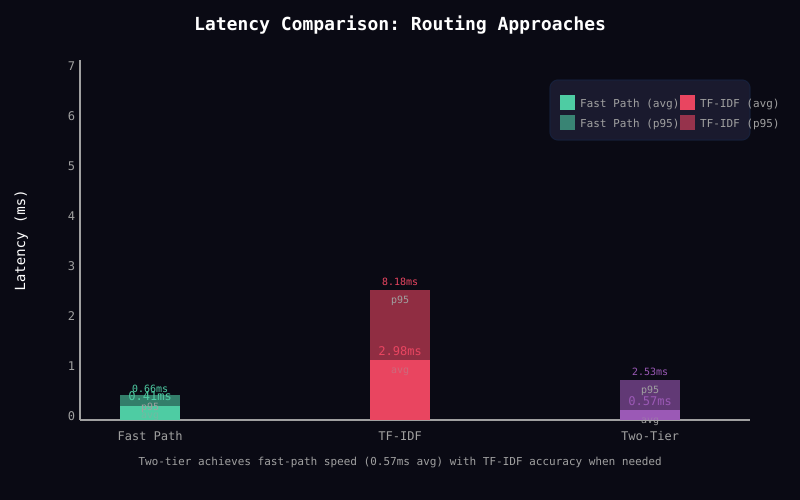
\includegraphics[width=0.9\textwidth]{../diagrams/07-latency-comparison.svg}
\caption{Latency comparison across routing approaches. Two-tier achieves fast-path speed (0.57ms avg) with TF-IDF accuracy when needed.}
\label{fig:latency}
\end{figure}

\begin{table}[h]
\centering
\begin{tabular}{lrrr}
\toprule
Metric & Fast Path & TF-IDF & Two-Tier \\
\midrule
Hit@1 & 0.400 & \textbf{0.600} & 0.420 \\
Hit@3 & 0.580 & \textbf{0.700} & 0.600 \\
Hit@5 & 0.660 & \textbf{0.740} & 0.680 \\
Recall@1 & 0.200 & \textbf{0.300} & 0.210 \\
Recall@3 & 0.340 & \textbf{0.400} & 0.350 \\
Recall@5 & 0.390 & \textbf{0.430} & 0.400 \\
MRR@10 & 0.507 & \textbf{0.659} & 0.524 \\
Latency avg (ms) & \textbf{0.41} & 2.98 & 0.57 \\
Latency p95 (ms) & \textbf{0.66} & 8.18 & 2.53 \\
\bottomrule
\end{tabular}
\caption{Routing metrics across three approaches}
\end{table}

\textbf{Key Findings:}
\begin{enumerate}
  \item TF-IDF alone achieves 60\% Hit@1, a 20-point improvement over fast path (40\%)
  \item Two-tier routing preserves fast-path speed (0.57ms avg) for 92\% of queries
  \item Token savings: 97.2\% reduction (7.6K index tokens vs 273K full-body tokens)
\end{enumerate}

\section{Discussion}

\textbf{Accuracy vs Speed Trade-off.} Our 60\% Hit@1 is lower than SkillRouter's 74\% on their 80K-skill benchmark, but our approach requires zero GPU and zero training. The 14-point gap is acceptable for many use cases, especially when GPU cost is considered.

\textbf{Two-Tier Efficiency.} The fast path handles 92\% of queries in <1ms. Only 8\% require TF-IDF fallback, keeping average latency at 0.57ms---comparable to fast path alone.

\textbf{Token Savings.} Loading all 156 SKILL.md files consumes 273K tokens. Our index uses 7.6K tokens (97.2\% reduction). For agents with limited context windows, this is the difference between loading 2 skills and loading all 156.

\textbf{Limitations.}
\begin{itemize}
  \item Our benchmark uses synthetic tasks; real user queries may have different distribution
  \item TF-IDF cannot capture semantic similarity (e.g., ``deploy'' $\to$ ``infrastructure'')
  \item The 156-skill registry is smaller than SkillRouter's 80K; scaling behavior is unknown
  \item Gold skill annotation was performed by a single author; inter-annotator agreement was not measured
\end{itemize}

\textbf{Future Work.}
\begin{itemize}
  \item Add embedding-based retrieval (e.g., sentence-transformers) as a third tier
  \item Expand benchmark to 500+ tasks with real user queries
  \item Evaluate cross-harness portability with Claude Code and Codex users
  \item Investigate adversarial skill injection resistance
  \item Conduct user study measuring agent task completion with/without routing
\end{itemize}

\section{Ethics Statement}

This work presents a tool selection system for LLM agents. The system does not collect user data, does not perform inference beyond routing decisions, and does not introduce new capabilities beyond selecting existing skills. Potential misuse includes: (1) adversarial skill injection to manipulate routing decisions, which we plan to investigate in future work; (2) over-reliance on automated tool selection without human oversight. We release all code and data to enable reproducibility and independent evaluation.

\section{Conclusion}

We present a two-tier skill routing architecture selecting relevant skills in <1ms on CPU with 97.2\% token savings. Our approach combines fast keyword matching with TF-IDF fallback, achieving 60\% Hit@1 without training. The system is harness-agnostic, working across OpenCode, Claude Code, and Codex. We release the registry format, router implementation, and benchmark as open source.

\bibliographystyle{plain}
\begin{thebibliography}{99}

\bibitem{skillrouter2026}
SkillRouter: Large Language Model-Based Skill Routing.
\newblock arXiv:2603.22455, July 2026.

\bibitem{masrouter2025}
MasRouter: Agentic Routing with Small Language Models.
\newblock ACL 2025.

\bibitem{routellm2025}
RouteLLM: Learning to Route LLMs with Preference Data.
\newblock ICLR 2025.

\bibitem{routerr12025}
Router-R1: Teaching LLMs to Reason via Reinforcement Learning.
\newblock NeurIPS 2025.

\bibitem{toolformer2023}
Schick, T., et al. Toolformer: Language Models Can Teach Themselves to Use Tools.
\newblock NeurIPS 2023.

\bibitem{gorilla2023}
Patil, S., et al. Gorilla: Large Language Model Connected with Massive APIs.
\newblock arXiv:2305.15334, 2023.

\bibitem{toolllm2024}
Qin, Y., et al. ToolLLM: Facilitating Large Language Models to Master 16000+ Real-world APIs.
\newblock ICLR 2024.

\bibitem{mcpzero2025}
MCP-Zero: Open-Source Tool Discovery for MCP.
\newblock arXiv:2506.01056, June 2025.

\bibitem{mcp2026}
Model Context Protocol Specification.
\newblock 2026-07-28.

\bibitem{anthropic2025}
Anthropic. Progressive Tool Loading: Reducing Context Bloat.
\newblock Internal Technical Report, 2025.

\bibitem{opencode}
OpenCode: AI-powered coding assistant.
\newblock \url{https://github.com/opencode-ai/opencode}

\bibitem{claudecode}
Claude Code: Anthropic's agentic coding tool.
\newblock \url{https://docs.anthropic.com/en/docs/claude-code}

\bibitem{codex}
Codex: OpenAI's cloud-based coding agent.
\newblock \url{https://openai.com/index/introducing-codex/}

\bibitem{lewis2020}
Lewis, P., et al. Retrieval-Augmented Generation for Knowledge-Intensive NLP Tasks.
\newblock NeurIPS 2020.

\bibitem{robertson2009}
Robertson, S. \& Zaragoza, H. The Probabilistic Relevance Framework: BM25 and Beyond.
\newblock Foundations and Trends in IR, 2009.

\bibitem{karpukhin2020}
Karpukhin, V., et al. Dense Passage Retrieval for Open-Domain Question Answering.
\newblock EMNLP 2020.

\bibitem{zhao2024}
Zhao, Y., et al. Lost in the Middle: How Language Models Use Long Contexts.
\newblock TACL 2024.

\bibitem{liu2023}
Liu, N., et al. Lost in the Middle: Language Models Use Long Contexts Poorly.
\newblock arXiv:2307.03172, 2023.

\bibitem{opencode-docs}
OpenCode Documentation. Skill System: Frontmatter and Loading.
\newblock \url{https://opencode.ai/docs/skills}

\end{thebibliography}

\end{document}
